\documentclass[12pt,letterpaper]{article}
\usepackage{graphicx,textcomp}
\usepackage{natbib}
\usepackage{setspace}
\usepackage{fullpage}
\usepackage{color}
\usepackage[reqno]{amsmath}
\usepackage{amsthm}
\usepackage{fancyvrb}
\usepackage{amssymb,enumerate}
\usepackage[all]{xy}
\usepackage{endnotes}
\usepackage{lscape}
\newtheorem{com}{Comment}
\usepackage{float}
\usepackage{hyperref}
\newtheorem{lem} {Lemma}
\newtheorem{prop}{Proposition}
\newtheorem{thm}{Theorem}
\newtheorem{defn}{Definition}
\newtheorem{cor}{Corollary}
\newtheorem{obs}{Observation}
\usepackage[compact]{titlesec}
\usepackage{dcolumn}
\usepackage{tikz}
\usetikzlibrary{arrows}
\usepackage{multirow}
\usepackage{xcolor}
\newcolumntype{.}{D{.}{.}{-1}}
\newcolumntype{d}[1]{D{.}{.}{#1}}
\definecolor{light-gray}{gray}{0.65}
\usepackage{url}
\usepackage{listings}
\usepackage{color}

\definecolor{codegreen}{rgb}{0,0.6,0}
\definecolor{codegray}{rgb}{0.5,0.5,0.5}
\definecolor{codepurple}{rgb}{0.58,0,0.82}
\definecolor{backcolour}{rgb}{0.95,0.95,0.92}

\lstdefinestyle{mystyle}{
	backgroundcolor=\color{backcolour},   
	commentstyle=\color{codegreen},
	keywordstyle=\color{magenta},
	numberstyle=\tiny\color{codegray},
	stringstyle=\color{codepurple},
	basicstyle=\footnotesize,
	breakatwhitespace=false,         
	breaklines=true,                 
	captionpos=b,                    
	keepspaces=true,                 
	numbers=left,                    
	numbersep=5pt,                  
	showspaces=false,                
	showstringspaces=false,
	showtabs=false,                  
	tabsize=2
}
\lstset{style=mystyle}
\newcommand{\Sref}[1]{Section~\ref{#1}}
\newtheorem{hyp}{Hypothesis}

\setcounter{secnumdepth}{0}

\title{Problem Set 2}
\date{Due: October 22, 2026}
\author{Barrera Munoz Diego}

\begin{document}
	\maketitle
	\tableofcontents
	\newpage
	
	\phantomsection
	\section{Question 1: Political Science}
	
	The following table was created using the data from a study run in a major Latin American city.\footnote{Fried, Lagunes, and Venkataramani (2010). ``Corruption and Inequality at the Crossroad: A Multimethod Study of Bribery and Discrimination in Latin America. \textit{Latin American Research Review}. 45 (1): 76-97.} As part of the experimental treatment in the study, one employee of the research team was chosen to make illegal left turns across traffic to draw the attention of the police officers on shift. Two employee drivers were upper class, two were lower class drivers, and the identity of the driver was randomly assigned per encounter. The researchers were interested in whether officers were more or less likely to solicit a bribe from drivers depending on their class (officers use phrases like, ``We can solve this the easy way'' to draw a bribe). The table below shows the resulting data.
	
	\begin{table}[h!]
		\centering
		\begin{tabular}{l | c c c }
			& Not Stopped & Bribe requested & Stopped/given warning \\
			\\[-1.8ex] 
			\hline \\[-1.8ex]
			Upper class & 14 & 6 & 7 \\
			Lower class & 7 & 7 & 1 \\
			\hline
		\end{tabular}
	\end{table}
	
	\begin{enumerate}
		\item [(a)] Calculate the $\chi^2$ test statistic by hand/manually (even better if you can do "by hand" in \texttt{R}).\\
		
		\vspace{.25cm}
		\textbf{Answer:} We will perform each calculation manually in R. 
		
		First we input our data in R.
		
		\lstinputlisting[language=R, firstline=9, lastline=12]{PS02_DBM.R}
		
		\begin{verbatim}
			Not stopped Bribe Warning
			Upper class          14     6       7
			Lower class           7     7       1
		\end{verbatim}
		
		\vspace{.25cm}
		
		Then we add the total for each column, row and the grand total.
		
		\lstinputlisting[language=R, firstline=15, lastline=22]{PS02_DBM.R}
		
		\lstinputlisting[language=R, firstline=24, lastline=28]{PS02_DBM.R}
		
		\begin{verbatim}
			Not stopped Bribe Warning Total
			Upper class          14     6       7    27
			Lower class           7     7       1    15
			Total                21    13       8    42
		\end{verbatim}
		
		\vspace{.25cm}
		Now we can calculate the expected count for each cell by multiplying the cell's row total by its column total and then divide it by the grand total. We repeat this calculation to all six cells in the table.
		
		\lstinputlisting[language=R, firstline=31, lastline=39]{PS02_DBM.R}
		
		\begin{verbatim}
			Not stopped  Bribe Warning
			Upper class        13.5 8.3571  5.1429
			Lower class         7.5 4.6429  2.8571
		\end{verbatim}
		
		\vspace{.25cm}
		
		Now, we follow this formula to get the chi-squared statistic:
		
		$$\chi^2 = \sum{\frac{(f_o -f_e)^2}{f_e}}$$
		
		First, we subtract each expected count from its observed count.
		
		\lstinputlisting[language=R, firstline=42, lastline=51]{PS02_DBM.R}
		
		\begin{verbatim}
			Not stopped   Bribe Warning
			Upper class         0.5 -2.3571  1.8571
			Lower class        -0.5  2.3571 -1.8571
		\end{verbatim}
		
		\vspace{.25cm}
		
		Now we square the difference. 
		
		\lstinputlisting[language=R, firstline=54, lastline=63]{PS02_DBM.R}
		
		\begin{verbatim}
			Not stopped  Bribe Warning
			Upper class        0.25 5.5561   3.449
			Lower class        0.25 5.5561   3.449
		\end{verbatim}
		
		\vspace{.25cm}
		
		Then, we divide by that cell's expected count.
		
		\lstinputlisting[language=R, firstline=66, lastline=75]{PS02_DBM.R}
		
		\begin{verbatim}
			Not stopped  Bribe Warning
			Upper class      0.0185 0.6648  0.6706
			Lower class      0.0333 1.1967  1.2071
		\end{verbatim}
		
		\vspace{.25cm}
		
		Finally, we add the six values.
		
		\lstinputlisting[language=R, firstline=78, lastline=79]{PS02_DBM.R}
		
		\begin{verbatim}
			Therefore, the chi-squared test statistic is: 3.791168
		\end{verbatim}
		
		\newpage
		\item [(b)] Now calculate the p-value from the test statistic you just created (in \texttt{R}).\footnote{Remember frequency should be $>$ 5 for all cells, but let's calculate the p-value here anyway.}  What do you conclude if $\alpha = 0.1$?\\
		
		\vspace{.25cm}
		\textbf{Answer:} First, we define our hypotheses:
		
		\begin{itemize}
			\item $H_0$: Driver's class and police response are independent.
			\item $H_a$: Driver's class and police response are associated.
		\end{itemize}
		
		We will need to calculate the degrees of freedom: $df=(2-1)(3-1)=2$. We use the upper tail of the chi-squared distribution:
		
		\lstinputlisting[language=R, firstline=85, lastline=87]{PS02_DBM.R}
		
		\begin{verbatim}
			The p-value is: 0.1502306
		\end{verbatim}
		
		Since $0.1502>0.10$, we \textbf{fail to reject the null hypothesis}.
		There is insufficient evidence with an $\alpha=0.1$ that police response is
		associated with driver's class. 
		
		Also, note that this does not establish independence. and that two of the six expected frequencies (4.643 and 2.857) are below 5, so the chi-squared approximation may be less reliable. Thus, this conclusion should be interpreted with caution.
		
		\newpage
		\item [(c)] Calculate the standardized residuals for each cell and put them in the table below.
		
		\vspace{.25cm}
		\textbf{Answer:} We calculate the standardized residuals with this formula:
		
		$$z_{ij}=\frac{O_{ij}-E_{ij}}{\sqrt{E_{ij}(1-p_{i\cdot})(1-p_{\cdot j})}}$$
		
		where $p_{i\cdot}$ is the row total divided by $n$ and $p_{\cdot j}$ is
		the column total divided by $n$.
		
		\vspace{.25cm}
		
		First, we calculate the two row proportions and three column proportions.
		
		\lstinputlisting[language=R, firstline=92, lastline=97]{PS02_DBM.R}
		
		Then, we calculate each cell's denominator by raising a value to
		the power $0.5$ to get its square root:
		
		\lstinputlisting[language=R, firstline=100, lastline=108]{PS02_DBM.R}
		
		Finally, we subtract the expected count from the observed count and divide
		by the corresponding denominator for each of the six values.
		
		\lstinputlisting[language=R, firstline=111, lastline=120]{PS02_DBM.R}
		
		The standardized residuals, rounded to three decimal places, are:
		
		\begin{center}
			\begin{tabular}{l | c c c}
				& Not stopped & Bribe requested & \shortstack{Stopped/given\\warning} \\
				\hline
				Upper class & $0.322$ & $-1.642$ & $1.523$ \\
				Lower class & $-0.322$ & $1.642$ & $-1.523$ \\
				\hline
			\end{tabular}
		\end{center}
		
		\newpage
		\item [(d)] How might the standardized residuals help you interpret the results?
		
		\vspace{.25cm}
		\textbf{Answer:} A positive residual means that the observed count is higher
		than expected under independence, and a negative residual means that it is lower. Also, a larger absolute residual indicates a larger standardized departure from independence.
		
		The largest departures occur in the bribe cells. Lower-class drivers
		were asked for bribes more often than expected ($z=1.642$), while upper-class drivers were asked less often than expected ($z=-1.642$).  Warnings show the opposite pattern: upper-class drivers received more warnings than expected, while lower-class drivers received fewer.
		
		The standarized residuals describe the direction of the observed pattern, but they do not overturn the overall test.
	\end{enumerate}
	
	\newpage
	\phantomsection
	\section{Question 2: Economics}
	
	Chattopadhyay and Duflo were interested in whether women promote different policies than men.\footnote{Chattopadhyay and Duflo. (2004). ``Women as Policy Makers: Evidence from a Randomized Policy Experiment in India. \textit{Econometrica}. 72 (5), 1409-1443.} Answering this question with observational data is pretty difficult due to potential confounding problems (e.g. the districts that choose female politicians are likely to systematically differ in other aspects too). Hence, they exploit a randomized policy experiment in India, where since the mid-1990s, $\frac{1}{3}$ of village council heads have been randomly reserved for women. A subset of the data from West Bengal can be found at the following link: \url{https://raw.githubusercontent.com/kosukeimai/qss/master/PREDICTION/women.csv}\\
	
	\noindent Each observation in the data set represents a village and there are two villages associated with one GP (i.e. a level of government is called "GP"). Figure 1 below shows the names and descriptions of the variables in the dataset. The authors hypothesize that female politicians are more likely to support policies female voters want. Researchers found that more women complain about the quality of drinking water than men. You need to estimate the effect of the reservation policy on the number of new or repaired drinking water facilities in the villages.
	
	\begin{center}
		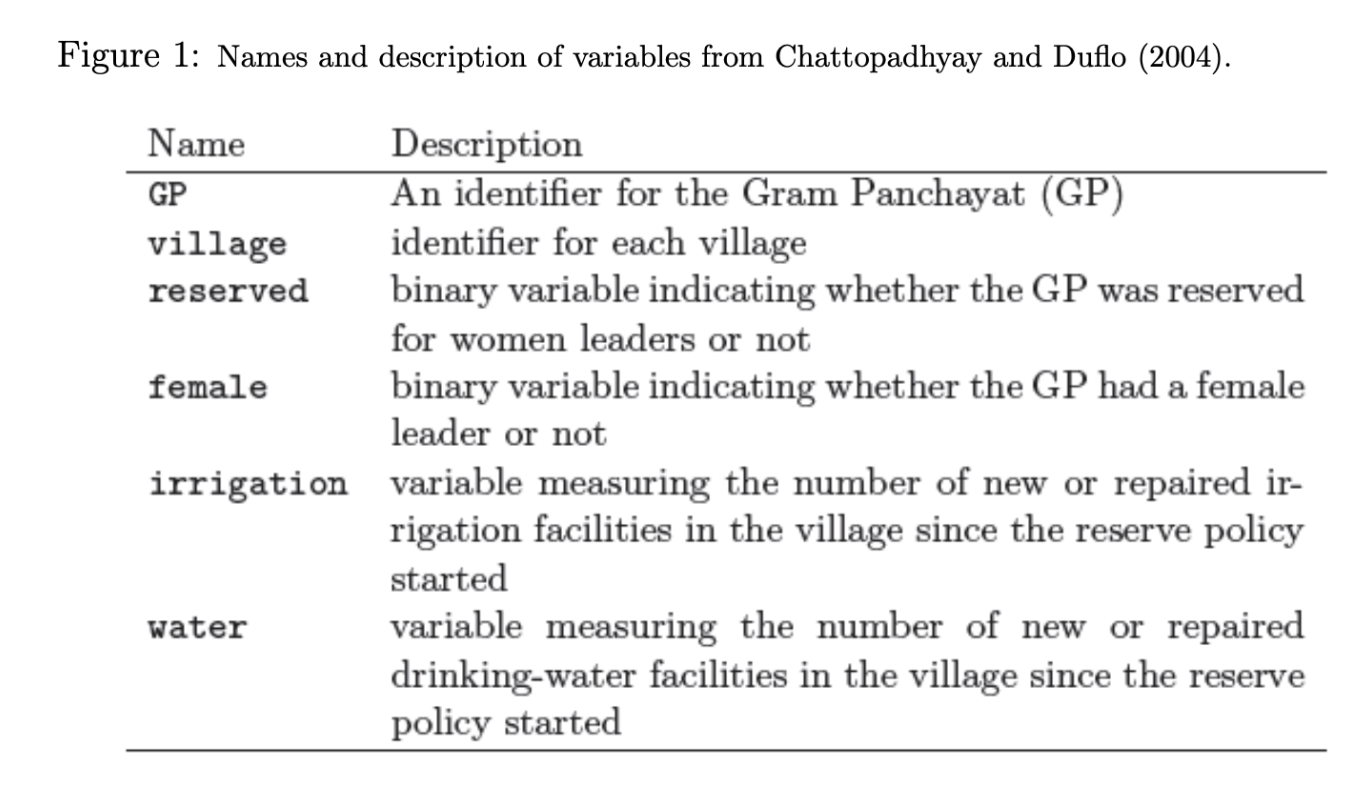
\includegraphics[width=\linewidth]{PS02_figures/figure_1.png}
	\end{center}
	
	\newpage
	
	\begin{enumerate}
		\item [(a)] State a null and alternative (two-tailed) hypothesis.
		
		\vspace{.25cm}
		\textbf{Answer:} Let $Y_i$ be the number of new or repaired drinking-water
		facilities in village $i$, and let $X_i=\texttt{reserved}_i$, where $X_i=1$
		if the GP was reserved for a female leader and $X_i=0$ otherwise.
		
		Our bivariate regression model would be:
		
		$$Y_i=\beta_0+\beta_1X_i+\varepsilon_i$$
		
		And the hypotheses are:
		\begin{itemize}
			\item $H_0:\beta_1=0$.
			\item $H_a:\beta_1\neq0$.
		\end{itemize}
		
		\vspace{.25cm}
		\item [(b)] Run a bivariate regression to test this hypothesis in \texttt{R}
		(include your code!).
		
		\vspace{.25cm}
		\textbf{Answer:} We will use \texttt{water} as the dependent variable and
		\texttt{reserved} as the explanatory variable. The policy is measured by
		\texttt{reserved} and \texttt{female} records whether the GP actually had a female leader. We will use $\alpha=0.05$ for this test statistic.
		
		First, we import the data and check their dimensions, missing values and
		reservation groups.
		
		\lstinputlisting[language=R, firstline=129, lastline=133]{PS02_DBM.R}
		
		The data contains 322 villages, six variables and no NAs. Also, there are 108 villages in reserved GPs and 214 in non-reserved GPs.
		
		\vspace{.25cm}
		Then we estimate the bivariate regression:
		
		\lstinputlisting[language=R, firstline=137, lastline=138]{PS02_DBM.R}
		
		The coefficient estimates from the regression output are:
		
		\begin{verbatim}
			Coefficients:
			Estimate Std. Error t value Pr(>|t|)    
			(Intercept)   14.738      2.286   6.446 4.22e-10 ***
			reserved       9.252      3.948   2.344   0.0197 *  
		\end{verbatim}
		
		\vspace{.25cm}
		
		Therefore, the fitted equation is:
		
		$$\widehat{Y}_i=14.7383+9.2524\,X_i$$
		
		For the reservation coefficient, the test statistic and degrees of freedom are:
		
		$$t=\frac{\hat\beta_1-0}{SE(\hat\beta_1)}=\frac{9.252423}{3.947746}=2.3437,\qquad df=322-2=320$$
		
		
		We reproduce the two-tailed test in R with this code:
		
		\lstinputlisting[language=R, firstline=141, lastline=146]{PS02_DBM.R}
		
		\begin{verbatim}
			t           df      p_value
			2.34372293 320.00000000   0.01970398
		\end{verbatim}
		
		\vspace{.25cm}
		
		Using $\alpha=0.05$, we \textbf{reject $H_0:\beta_1=0$}. Under the usual OLS assumptions, there is evidence that the mean number of new or repaired drinking-water facilities differs between reserved and non-reserved GPs.
		
		The 95\% confidence interval for the policy coefficient is given by:
		
		$$\beta_1\pm t_{0.975,320}\,SE(\hat\beta_1)=9.2524\pm1.9674(3.9477)$$
		
		We obtain the interval in R using the following code:
		
		\lstinputlisting[language=R, firstline=149, lastline=152]{PS02_DBM.R}
		
		\begin{verbatim}
			Lower     Upper 
			1.485608 17.019238 
		\end{verbatim}
		
		\vspace{.25cm}
		
		These are conventional OLS standard errors, which assume independent errors with constant variance. The two villages in the same GP may have related errors, so the reported p-value and interval depend on these assumptions.
		
		We can also visualize the difference using the plot below, which shows the OLS fitted mean number of new or repaired drinking-water facilities for each group, together with the corresponding 95\% confidence intervals.
		
		\lstinputlisting[language=R, firstline=158, lastline=171]{PS02_DBM.R}
		
		\begin{center}
			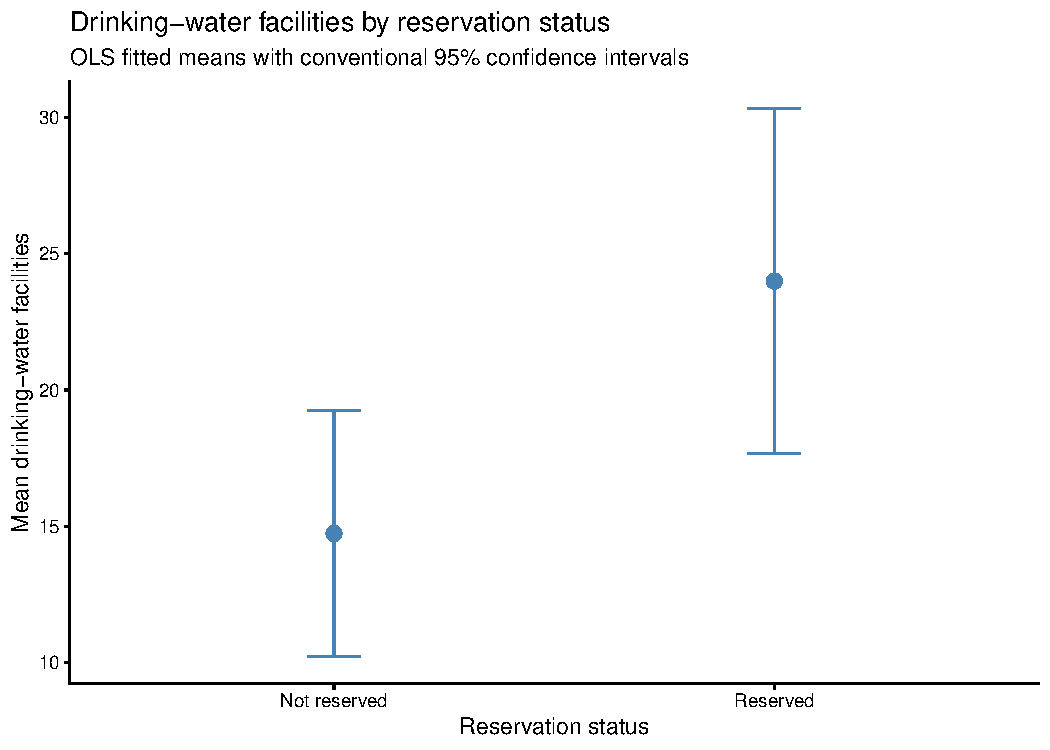
\includegraphics[width=\linewidth]{PS02_figures/PS02_group_means.pdf}
		\end{center}
		
		\newpage
		\item [(c)] Interpret the coefficient estimate for the reservation policy.
		
		\vspace{.25cm}
		
		\textbf{Answer:} The coefficient is $\hat\beta_1=9.2524$. Villages in reserved
		GPs have an estimated $9.25$ more new or repaired drinking-water
		facilities per village, on average, than villages in non-reserved GPs.
		
		Because \texttt{reserved} is defined as 0/1, the coefficient is the difference
		between the two sample means. We can calculate these means in R using this code:
		
		\lstinputlisting[language=R, firstline=177, lastline=178]{PS02_DBM.R}
		
		\begin{verbatim}
			0        1
			14.73832 23.99074
		\end{verbatim}
		
		The estimated mean for villages in non-reserved GPs is $14.7383$ facilities.
		For villages in reserved GPs, it is $23.9907$. Therefore,
		
		$$\bar Y_1-\bar Y_0=23.9907-14.7383=9.2524$$
		
		In R code:
		
		\lstinputlisting[language=R, firstline=179, lastline=180]{PS02_DBM.R}

		\begin{verbatim}
		[1] 9.252423
		\end{verbatim}
		
		The intercept is the estimated mean for villages in non-reserved GPs.
		Since reservation was randomly assigned, this difference supports interpreting
		$9.25$ as an estimate of the average causal effect of the reservation policy.
		It is a difference in the number of facilities per village, not a percentage.
		
	\end{enumerate}
\end{document}